%----------------------------------------------------------------------------------------
%	PACKAGES AND THEMES
%----------------------------------------------------------------------------------------
\PassOptionsToPackage{table}{xcolor}
\documentclass[aspectratio=169,xcolor=dvipsnames,svgnames,x11names,fleqn]{beamer}
% \documentclass[aspectratio=169,xcolor=dvipsnames,fleqn]{beamer}

\usetheme{RedVelvet}

\usefonttheme[onlymath]{serif}
\newcommand{\showanswers}{yes}


\usepackage{xspace}
\usepackage{amsmath}
\usepackage{amssymb}
\usepackage{amsfonts}
\usepackage{color}
\usepackage{physics}
% \usepackage{mathbb}
\usepackage{rahul_math}
\usepackage{bigints}

\usepackage{graphicx} % Allows including images
\usepackage{booktabs} % Allows the use of \toprule, \midrule and \bottomrule in tables
\usepackage{tikz,pgfplots}

\usepackage{subfigure}
\usetikzlibrary{arrows}
\usepackage{minted}
\definecolor{LightGray}{gray}{0.9}
\definecolor{cream}{rgb}{0.92, 0.9, 0.55}
\definecolor{lightblue}{rgb}{0.68, 0.85, 0.9}


\usepackage{xcolor-material}
\usetikzlibrary{fit}
\usetikzlibrary{matrix}
\tikzset{%
apple/.pic={
    \fill [MaterialBrown] (-1/8,0)  arc (180:120:1 and 3/2) coordinate [pos=3/5] (@)-- ++(1/6,-1/7)  arc (120:180:5/4 and 3/2) -- cycle;
    \fill [MaterialLightGreen500] (0,-9/10)  .. controls ++(180:1/8) and ++(  0:1/4) .. (-1/3,  -1) .. controls ++(180:1/3) and ++(270:1/2) .. (  -1,   0) .. controls ++( 90:1/3) and ++(180:1/3) .. (-1/2, 3/4) .. controls ++(  0:1/8) and ++(135:1/8) .. (   0, 4/7)
    }
    }

\newcommand{\leftdoublequote}{\textcolor{blue}{\scalebox{3}{``}}}

\newcommand{\rightdoublequote}{\textcolor{blue}{\scalebox{3}{''}}}


\usepackage{textcomp}
\usepackage{fontawesome}
\usepackage{tikz,pgfplots}
\usetikzlibrary{shapes.callouts}
\usetikzlibrary{arrows}


\usepackage{overpic}

%----------------------------------------------------------------------------------------
%	TITLE PAGE
%----------------------------------------------------------------------------------------

\usepackage{tikz-qtree,tikz-qtree-compat}
\usetikzlibrary{tikzmark}
\usetikzlibrary{calc}


\title[CPE 486/586: Machine Learning]{CPE 486/586: Machine Learning for Engineers} % The short title appears at the bottom of every slide, the full title is only on the title page
\subtitle{07 Advanced Regression}

\author[Rahul Bhadani] {{\Large \textbf{Rahul Bhadani}}}

\institute[UAH] % Your institution as it will appear on the bottom of every slide, maybe shorthand to save space
{
    Electrical \& Computer Engineering,  The University of Alabama in Huntsville
}
\date

% \titlegraphic{
%    \includegraphics[width=0.4\linewidth]{figures/UAH_primary.png}
% }

\begin{document}

%-------------------------------------------------
\begin{frame}
    \titlepage
\end{frame}

%-------------------------------------------------
\begin{frame}{Outline}
    \backgroundtableofcontents
\end{frame}



  %%%%%%%%%%%%%%%%%%%%%%%%%%%%%%%%%%%%%%%%%%%%%%%%%%%%%
\begin{sectionframe}{\faGroup}{Polynomial Regression}
\end{sectionframe}

\begin{frame}[allowframebreaks]{Polynomial Regression}
\Large
    \begin{tblock}{Regression Model}
        \begin{equation}
            y_i = w_0 + w_1 x_{i} + w_2 x_{i}^2 + \cdots  + w_k x_{i}^k + \epsilon_i
        \end{equation}
    \end{tblock}
    
    In this model, we only have single feature.
\end{frame}
    
    
\begin{frame}[allowframebreaks]{Vectorizing Polynomial Regression}

    \begin{tblock}{Regression Model}
        \begin{equation}
            \begin{bmatrix}
                y_1 \\ y_2 \\ \vdots \\y_n 
            \end{bmatrix} = \begin{bmatrix}
                1 & x_1 & x_1^2 & \cdots x_1^k\\
                1 & x_2 & x_2^2 & \cdots x_2^k\\
                \cdots & \cdots & \cdots & \cdots \cdots\\
                1 & x_n & x_n^2 & \cdots x_n^k
            \end{bmatrix}
            \begin{bmatrix}
                w_1 \\ w_2 \\ \vdots \\w_k 
            \end{bmatrix} + \begin{bmatrix}
                \epsilon_1 \\ \epsilon_2 \\ \vdots \epsilon_n 
            \end{bmatrix} \Rightarrow \ybf = \Xbf \wbf + \boldsymbol{\epsilon}
        \end{equation}
    \end{tblock}
    
    
        $\Xbf$ is called the Vandermonde matrix (this is different from $\Xbf$ obtained in the matrix form of the MLR model).

    \end{frame}
    

    \begin{frame}{Least Square Solution}

        To find, $\wbf$, 

        \begin{multiequation}
            \ybf  & = \Xbf \wbf\\
            \Xbf^\top \Xbf \wbf & = \Xbf^\top \ybf
        \end{multiequation}

        Then, the ordinary least square estimate provides the solution as
        $$
        \hat{\wbf} = (\Xbf^\top \Xbf)^{-1}\Xbf^\top \ybf.
        $$
    
    Polynomial regression can be expanded to multiple features.
    \end{frame}

\begin{frame}{Fitted Values and Residuals}
    
    The residual term is
    \begin{multiequation}
        \ebf_{n\times 1} = \ybf - \hat{\ybf} = \ybf - \Xbf \hat{\wbf}
    \end{multiequation}

The vector of the fitted value $\hat{\ybf}$ can be expressed in terms of the hat matrix $\Hbf$ as

\begin{multiequation}
    \hat{\ybf}_{n\times 1} = \Hbf \ybf
\end{multiequation}

where 
\begin{multiequation}
    \Hbf_{n\times n} = \Xbf ( \Xbf^\top \Xbf)^{-1} \Xbf^\top
\end{multiequation}

Then, we could also write $ \ebf_{n\times 1} = (\Ibf - \Hbf)\Ybf$.

\end{frame}

\begin{frame}{Polynomial Model with Multiple Features}

    Polynomial Regression can also expand to multiple features:
    \begin{multiequation}
        y_i = w_0 + w_1\times area + w_2 \times (area)^2 + w_3 \times num\_rooms + w_4 \times yard\_sqft
    \end{multiequation}
\end{frame}


%%%%%%%%%%%%%%%%%%%%%%%%%%%%%%%%%%%%%%%%%%%%%%%%%%%%%
\begin{sectionframe}{\faGavel}{Locally Weighted Kernel Regression}
\end{sectionframe}


    %------------------------------------------------
    \begin{frame}{Intuition}
    
    \begin{center}
        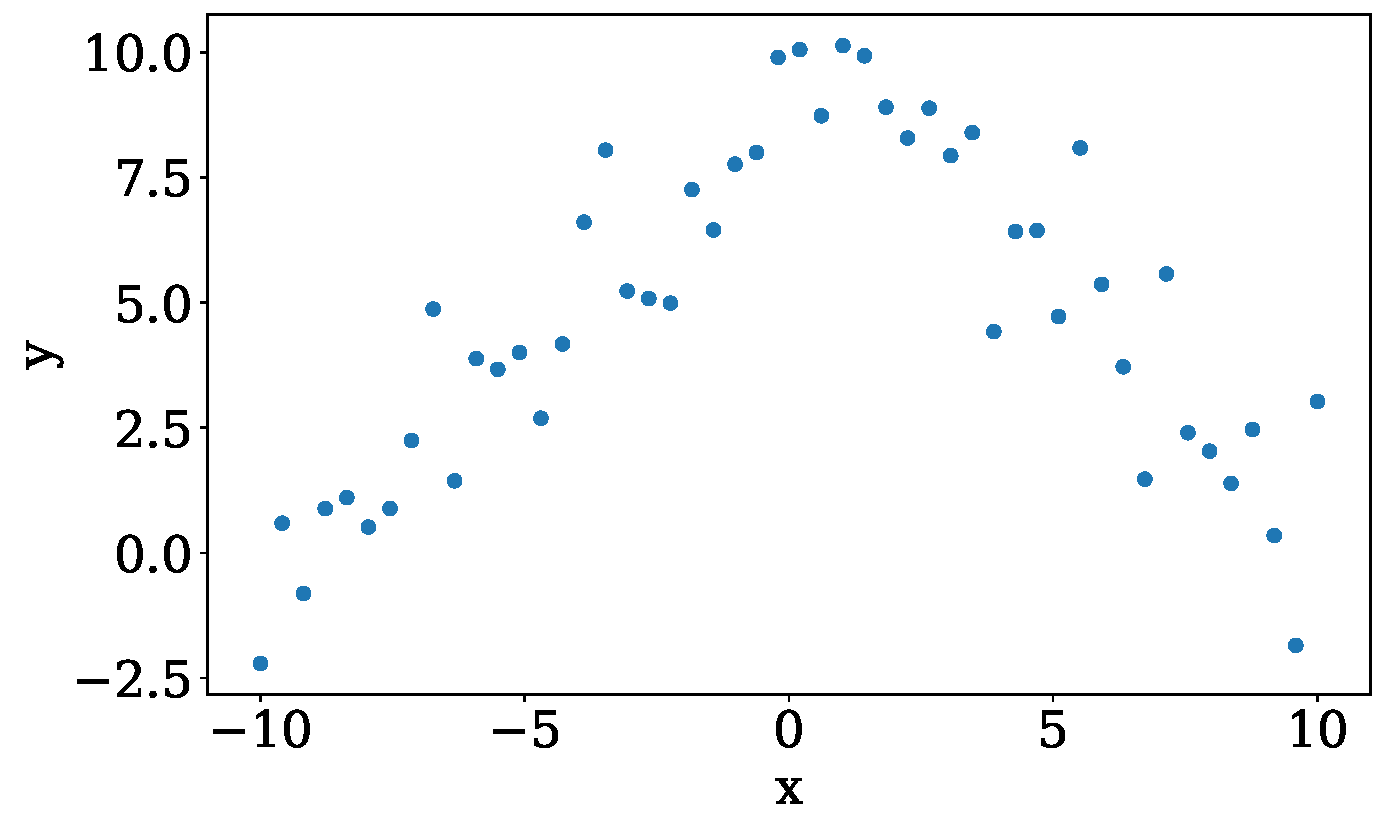
\includegraphics[width=0.50\textwidth]{figures/inverted_v.pdf}
    \end{center}
\end{frame}

\begin{frame}{Intuition}
    
    \begin{center}
        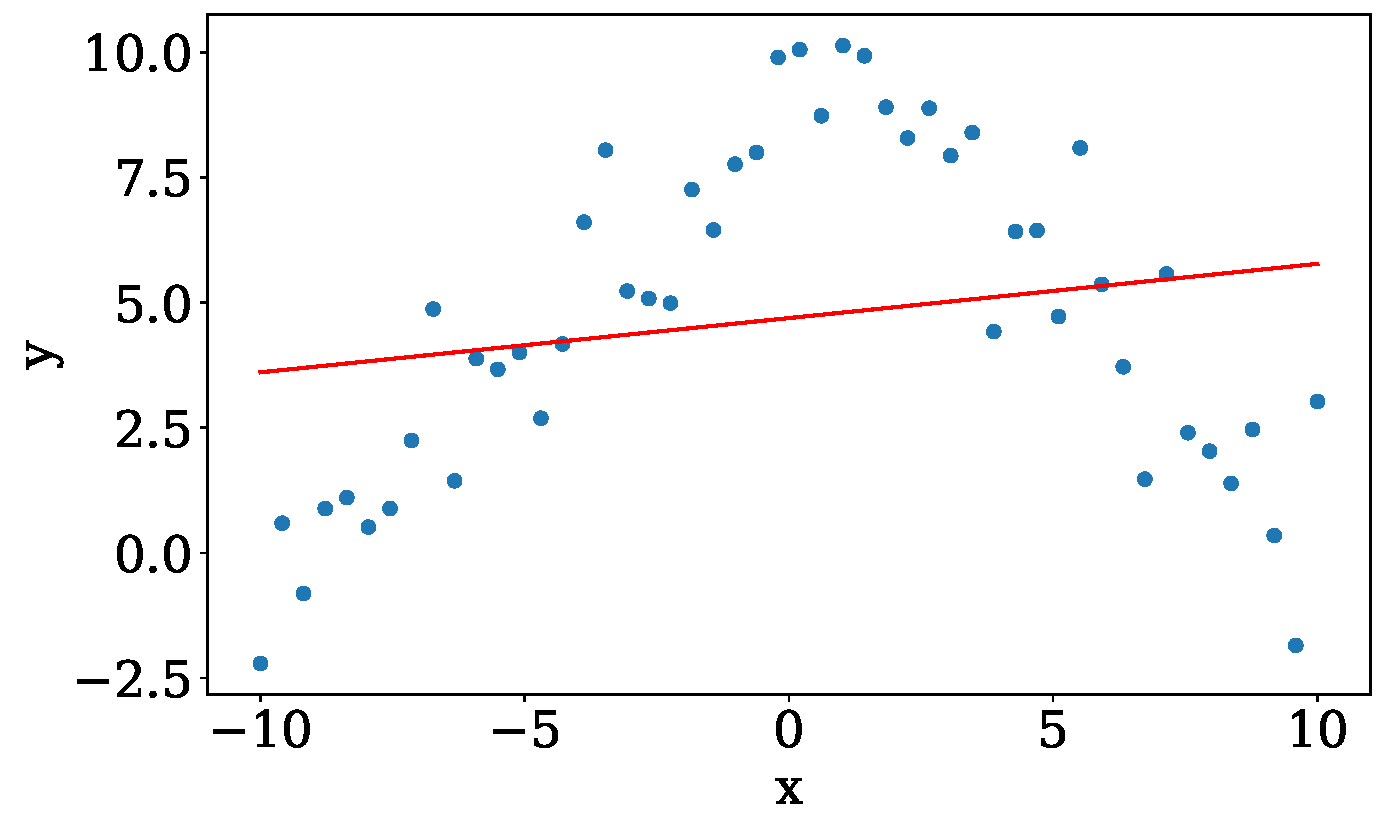
\includegraphics[width=0.50\textwidth]{figures/inverted_v_fit.pdf}
    \end{center}
\end{frame}

\begin{frame}{Intuition}
    \begin{center}
    \LARGE
    Clearly, here are two sets of data points.
    \end{center}
\end{frame}

\begin{frame}{Intuition}
    \begin{center}
    \LARGE
    We may benefit from fitting two kinds of regression lines. That can be done using a locally-weighted regression line.
    \end{center}
\end{frame}

\begin{frame}{Locally Weighted Kernel Regression}
    \begin{tblock}{Implementing Locally Weighted Regression}
        \begin{enumerate}
            \item Provide a smoothing parameter $h$.
            \item Provide a degree of polynomial fit (if you are doing polynomial fit).
            \item Select some query points.
        \end{enumerate}
    \end{tblock}
\end{frame}

\begin{frame}{Cost Function for Locally Weight Kernel Regression}
    \begin{tblock}{Cost Function}
        \begin{multiequation}
            J(\wbf) = \cfrac{1}{2n}( \ybf - \xbf\wbf)^\top \boldsymbol{\kappa}( \ybf - \xbf\wbf)
        \end{multiequation}
        where 
        \begin{multiequation}
            \boldsymbol{\kappa} = \begin{bmatrix}
                \kappa_1 & 0 & \cdots & 0\\
                0 & \kappa_1 & \cdots & 0\\
                \vdots & \vdots & \vdots & \vdots\\
                0 & 0 & 0 & \kappa_n
            \end{bmatrix}
        \end{multiequation} is a \textbf{kernel function}.
    \end{tblock}
\end{frame}


\begin{frame}{Estimator}

    \begin{tblock}{Closed Form of Estimation}
    \begin{equation}
        \wbf =\tfrac{1}{n} (\xbf \boldsymbol{\kappa}\xbf)^{-1}\xbf^\top \wbf \ybf
    \end{equation} 
    \end{tblock}

    \large 
    This method is also called \textbf{Lowess (locally weighted regression scatter plot smoothing)} or \textbf{Loess}.
\end{frame}

    % %------------------------------------------------
    
\begin{frame}{Choosing a Kernel Function}

    \begin{center}
        \large
    The basic idea of kernel regression is that in estimating the model $f$, when we want to fit a regression line in the vicnity of $x_0$,  it is desirable to give greater  weight to observations that are close to the pivot $x_0$.
    \end{center}

\end{frame}

\begin{frame}{Choosing a Kernel Function}


    \begin{center}
        \large 

        We first stanardize the predictor variable $x$ as $z = \cfrac{x-x_0}{h}$ where $x_0$ is pivot point, and $h$ is called kernel bandwidth (which is a design choice).

        \begin{tblock}{}
            We need a kernel function $\kappa(z)$ that attaches greatest weight to observations that are close to the focal $x_0$ and then falls off symmetrically and smoothly as $|z|$ grows.
        \end{tblock}
    \end{center}
\end{frame}

\begin{frame}{Some Kernel Functions}
\begin{center}
    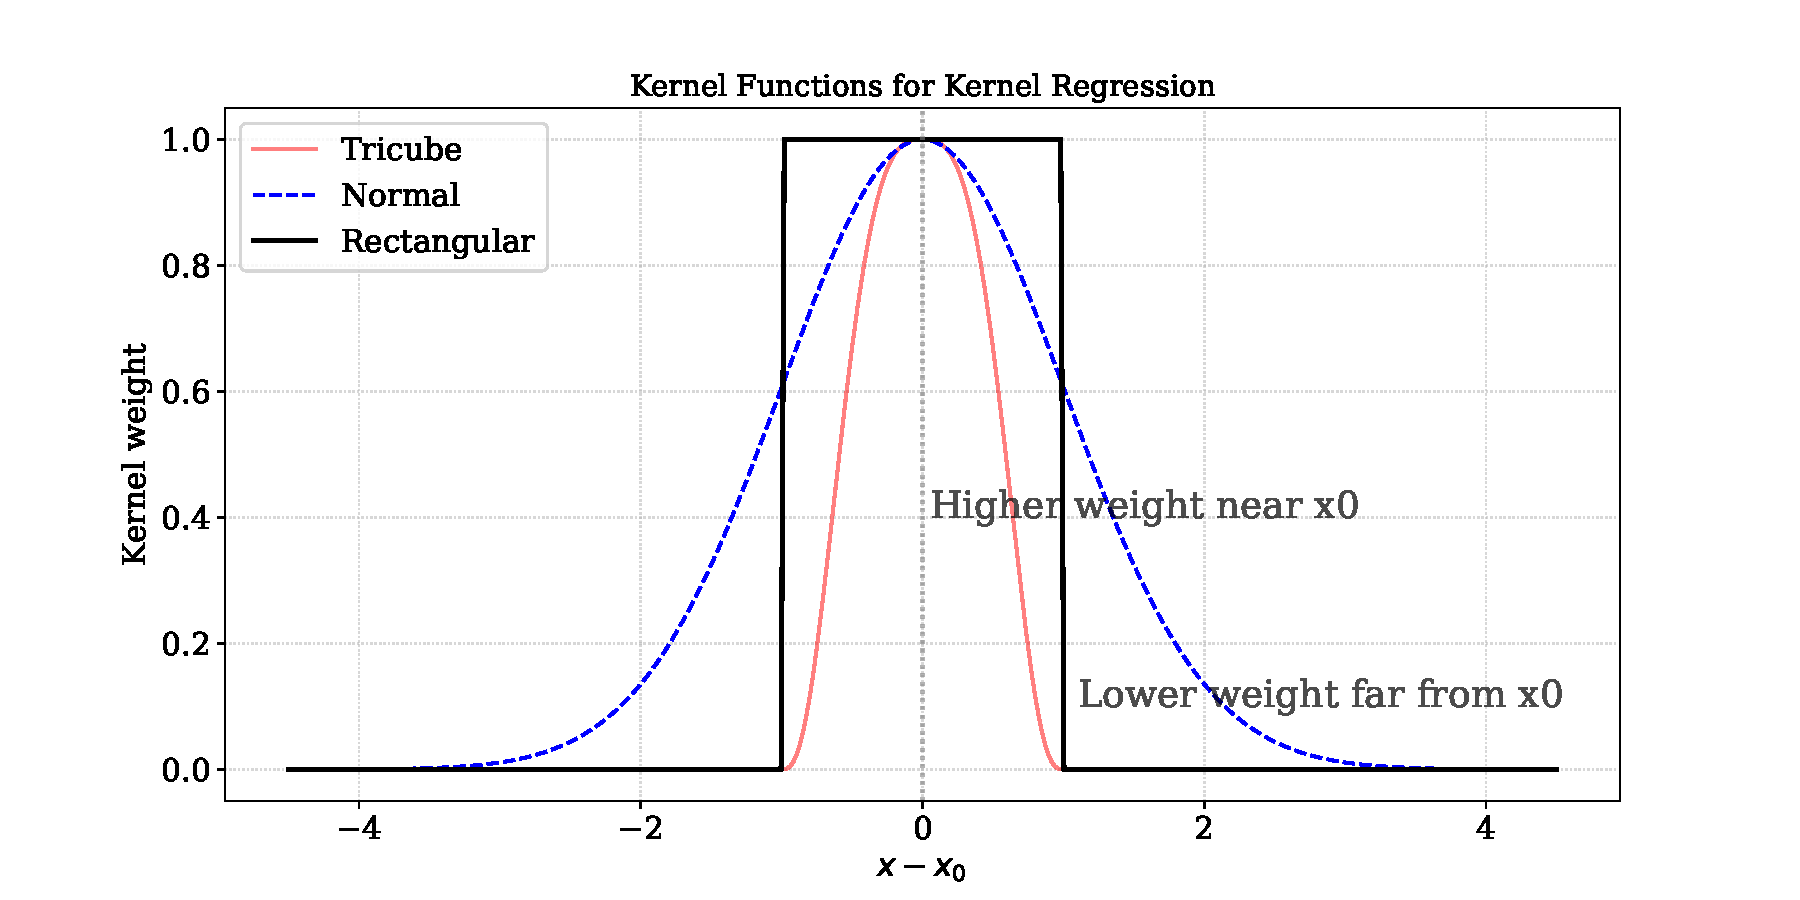
\includegraphics[width=0.90\textwidth]{figures/loess_kernel.pdf}
\end{center}
\end{frame}
    
    \begin{frame}{Gaussian Kernel}

        One popular kernel function for the LWR is Gaussian function (also known as radial basis function (RBF) ):
    
        The radial kernel (Radial Basis Function (RBF)) is a Gaussian function, a popular measure of similarity between two data points, and it decreases with the distance ranging from $0$ to $1$.
    $1$ means two points are identical.
    
    RBF between two points $x$ and $x_0$ is defined as
    
    $$
    \kappa(x, x_0) = \exp\bigg( -\cfrac{||x-x_0||^2}{2h^2} \bigg)
    $$\
    where $h$ is the bandwidth of the kernel function.
    \end{frame}
    
    \begin{frame}{The Tricube Kernel}

        \begin{tblock}{}
            
            \begin{multiequation}
                \kappa(z) = \begin{cases}
                    (1  - |z|^3)^3 & \quad |z|  < 1\\
                    0 & \quad |z| \geq 1
                \end{cases}
            \end{multiequation}

        \end{tblock}
        
    \end{frame}

    \begin{frame}{The Rectangular Kernel}

        \begin{tblock}{}
            
            \begin{multiequation}
                \kappa(z) = \begin{cases}
                    1 & \quad |z|  < 1\\
                    0 & \quad |z| \geq 1
                \end{cases}
            \end{multiequation}

        \end{tblock}
        
    \end{frame}

    \begin{frame}{Steps in Implementing Loess}
        \begin{itemize}
            \item Provide smoothing value, $h$
            \item Provide degree of $\wbf$ for the polynomial fit
            \item Select pivot point(s) $x_0$.
        \end{itemize}
    \end{frame}

    \begin{frame}{Additional Reading and Reference}
        
        \Large
\begin{center}
    Chapter 18, Applied Regression Analysis and Generalized Linear Models, John Fox, Third Edition, SAGE Publications, Inc.
\end{center}

    \end{frame}

    \begin{frame}{Classwork}

        \begin{itemize}
            \item  For Loess, if we choose a different pivot point $x_0$, what computation can be reused? 
            \item  What do we need to store vs what we can compute for a new pivot point?
        \end{itemize}

    \end{frame}

% https://jeffmacaluso.github.io/post/LinearRegressionAssumptions/
% https://www.kirenz.com/blog/posts/2021-11-14-linear-regression-diagnostics-in-python/
% https://medium.com/@sahin.samia/ml-series-3-regression-assumption-check-ensuring-the-validity-of-linear-regression-models-using-5d876394ae81


%%%%%%%%%%%%%%%%%%%%%%%%%%%%%%%%%%%%%%%%%%%%%%%%%%%%%
\begin{sectionframe}{\faGroup}{Model Diagnostics and Assumption Checking}
\end{sectionframe}

\begin{frame}{Assumptions in Linear Regression}
    \begin{enumerate}
        \item Linearity
        \item Additivity
        \item Normality of the Error Terms
        \item No Multicollinearity among Predictors
        \item No Autocorrelation of the Error Terms
        \item Homoscedasticity
    \end{enumerate}
\end{frame}

\begin{frame}{Residual Plot Analysis}

    \Large 
    \begin{itemize}
        \item   $e = \yhat - y$ vs $x$ is called residual plot.
        \item     Residual plot provides a valuable information about assumption validation.

    \end{itemize}
  

\end{frame}

\begin{frame}{Linearity Assumption in Linear Regression}
    Simple Linear Regression assumes that there is linear relationship between the predictors (e.g. independent variables or features) and the response variable (e.g. dependent variable or label).

    \begin{tblock}{How to detect the violation of linearity?}
        \begin{itemize}
            \item Coefficient of Determination
            \item Plot the data 
        \end{itemize}
    \end{tblock}
\end{frame}


\begin{frame}{Additivity Assumption in Linear Regression}
    Additivity assumes that the impact of different predictors is additive.
    For example, consider
    $$
    y = w_0 + w_1 x_1 + w_2 x_2 + \epsilon
    $$
    Additivity says that changing a predictor by some amount will contribute to change in the response in similar proportion.

    Example: Let $\tilde{x}_2 = x_2 + 1$, then

    \begin{multiequation}
        \tilde{y} & =  w_0 + w_1 x_1 + w_2 \tilde{x}_2 + \epsilon\\
        & =  w_0 + w_1 x_1 + w_2 (x_2 + 1) + \epsilon\\
        & =  (w_0 + w_1 x_1 + w_2 x_2 + \epsilon) + w_2\\
        & = y + w_2
    \end{multiequation}
    Hence, we see incremental change in $x_2$ causes incremental change in $y$.
\end{frame}

\begin{frame}{Additivity Violation}
    \begin{columns}
        \column{0.5\linewidth}
        Additivity violation occur when there is interaction term in the true model or a higher order term(.e.g. $x_1 x_2$, or $x_2^2$ ) that we didn't consider. We can plot correlation matrix to check for additivity violation.
        \column{0.5\linewidth}
        \begin{center}
            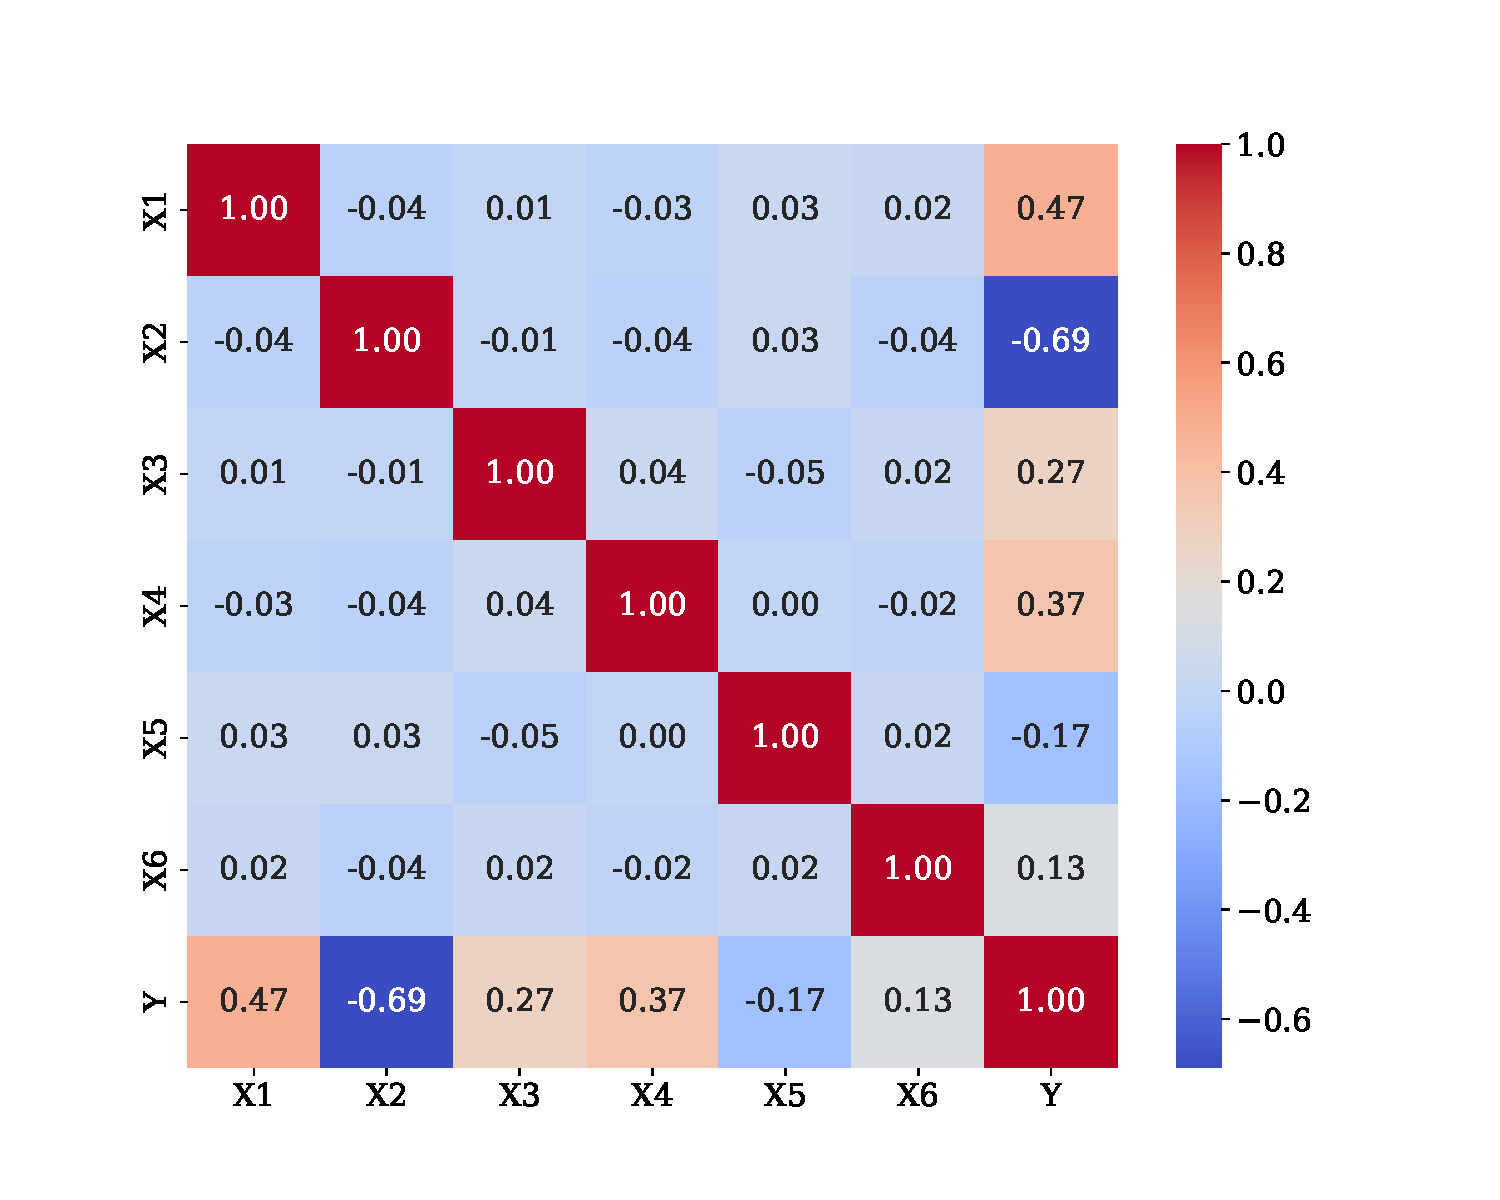
\includegraphics[width=1.0\textwidth]{figures/heatmap_interaction.pdf}
        \end{center}
    \end{columns}
\end{frame}


\begin{frame}{Normality Assumptions}
    \large
    \begin{columns}
        \column{0.5\linewidth}
        \begin{itemize}
            \item     We assume that error are zero mean constant variance Gaussian distribution.
            \item Scatter plot of residual, and density estimation plot should exhibit any deviation from normality.
        \end{itemize}
        \column{0.5\linewidth}
        \begin{center}
            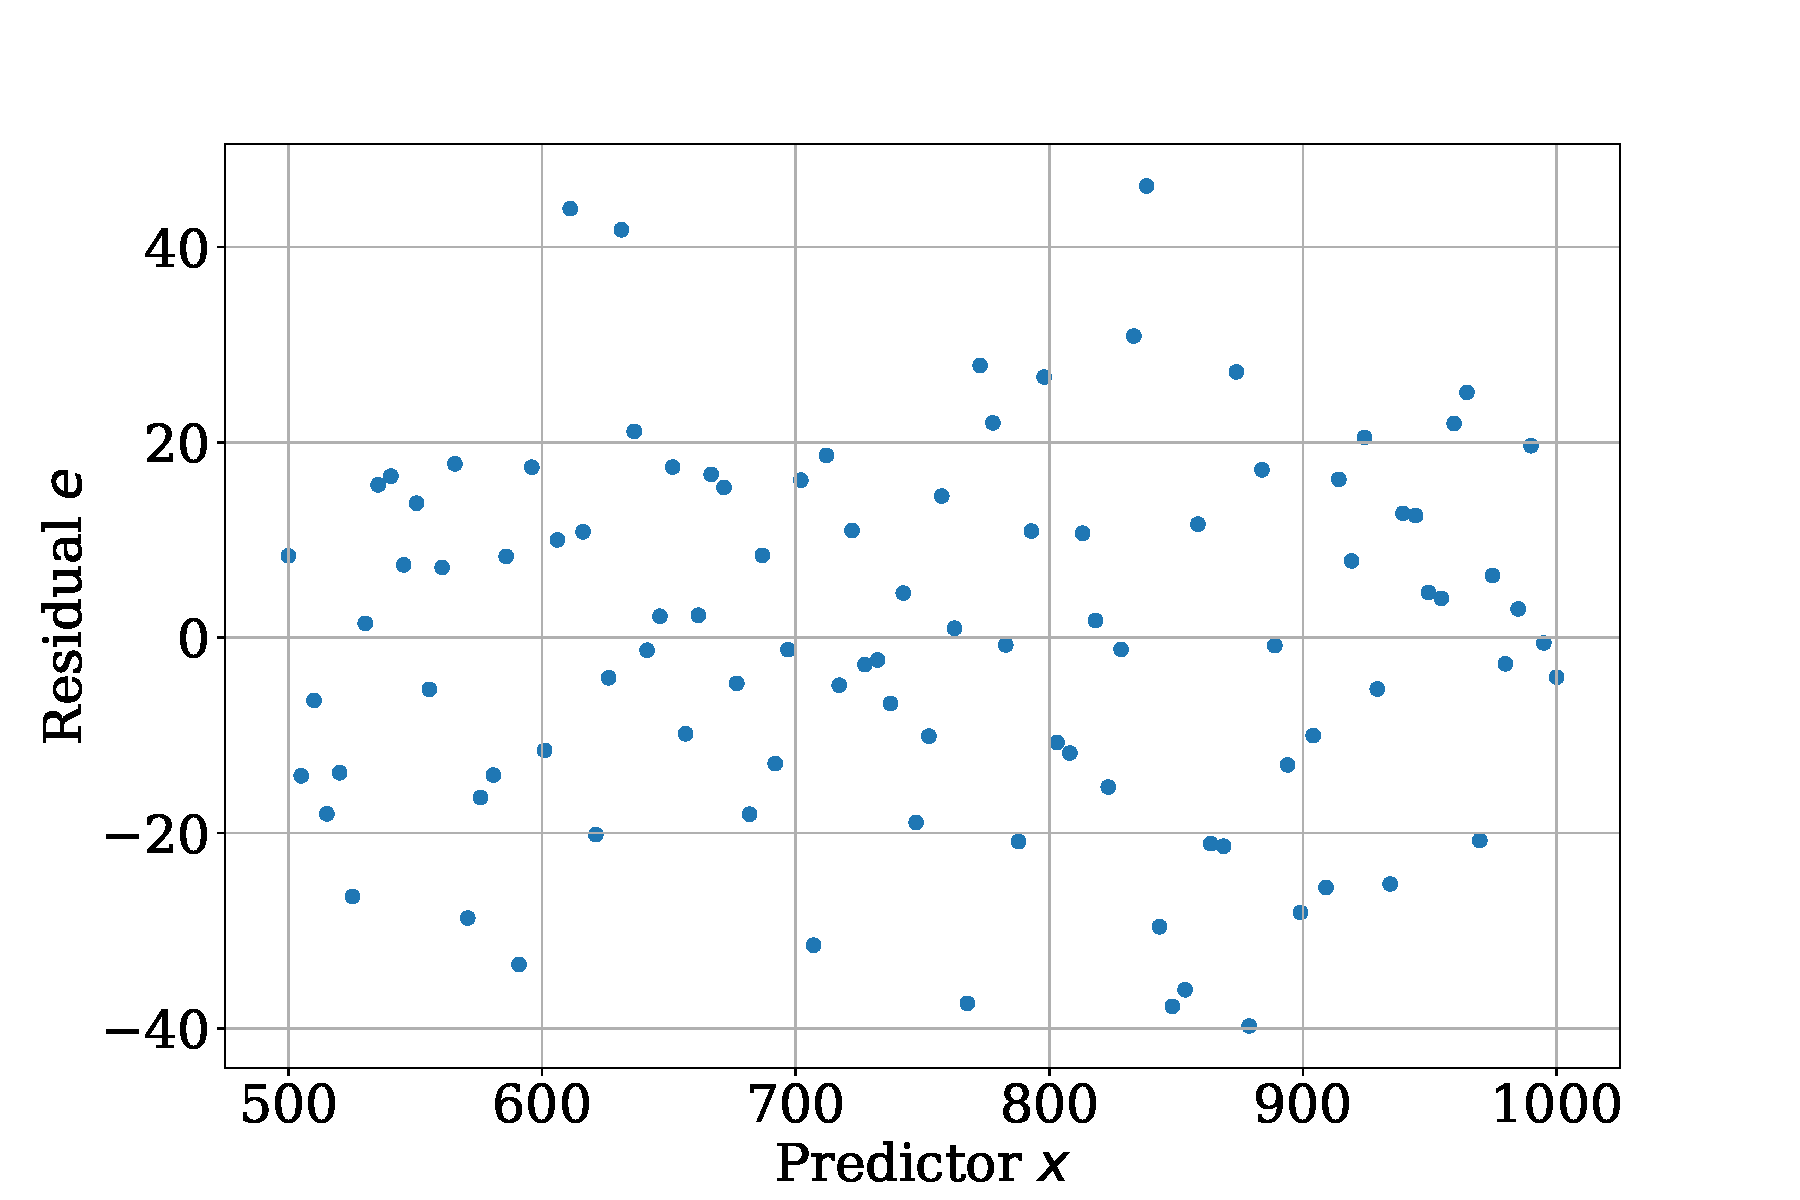
\includegraphics[width=1.0\textwidth]{figures/normal_residual_plot.pdf}

            \textit{Follows the normality assumption}
        \end{center}
    \end{columns}
    
\end{frame}


\begin{frame}{QQ-plot for Normality}
    \large
    \begin{columns}
        \column{0.5\linewidth}
        \begin{itemize}
            \item    A Q-Q plot (Quantile-Quantile plot) can help in assessing normality assumption.
            \item  It compares the quantiles of the residuals from the regression model with the quantiles of a theoretical normal distribution.
        \end{itemize}
        \column{0.5\linewidth}
        \begin{center}
            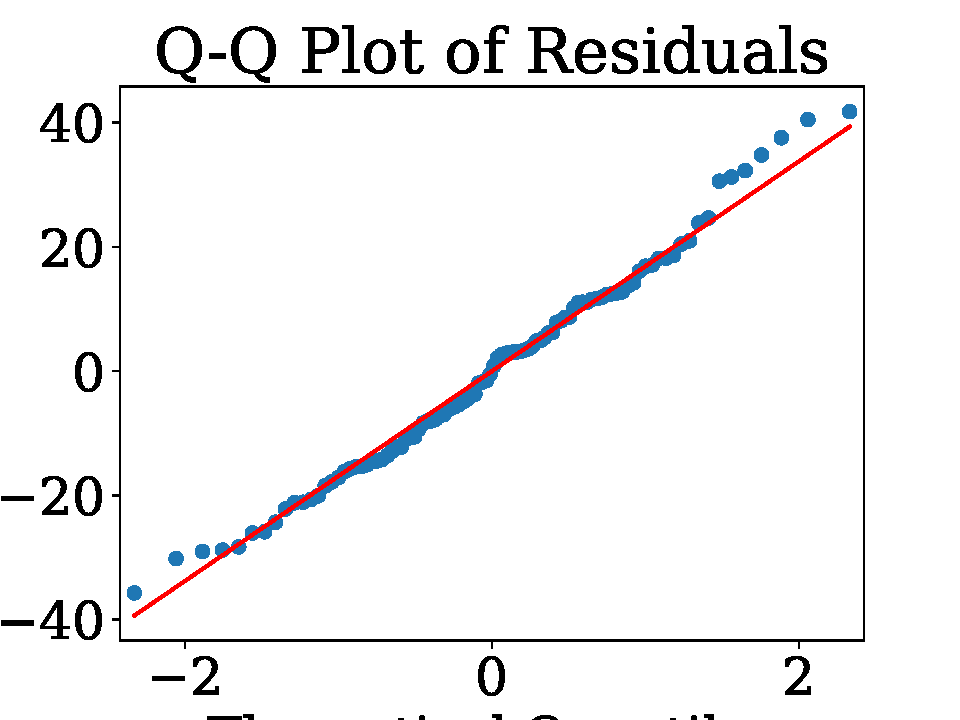
\includegraphics[width=0.8\textwidth]{figures/qq_plot.pdf}

            \textit{Follows the normality assumption}
        \end{center}
    \end{columns}
    
\end{frame}

\begin{frame}{Multicollinearity}
     \large
    \begin{columns}
        \column{0.4\linewidth}
        \begin{itemize}
            \item      In case of multiple regression, if predictor variables are correlated, multicollinearity among them is said to exist.

    \item Plot the scatterplot  matrix to check for multicollinearity.
        \end{itemize}
        \column{0.6\linewidth}
        \begin{center}
            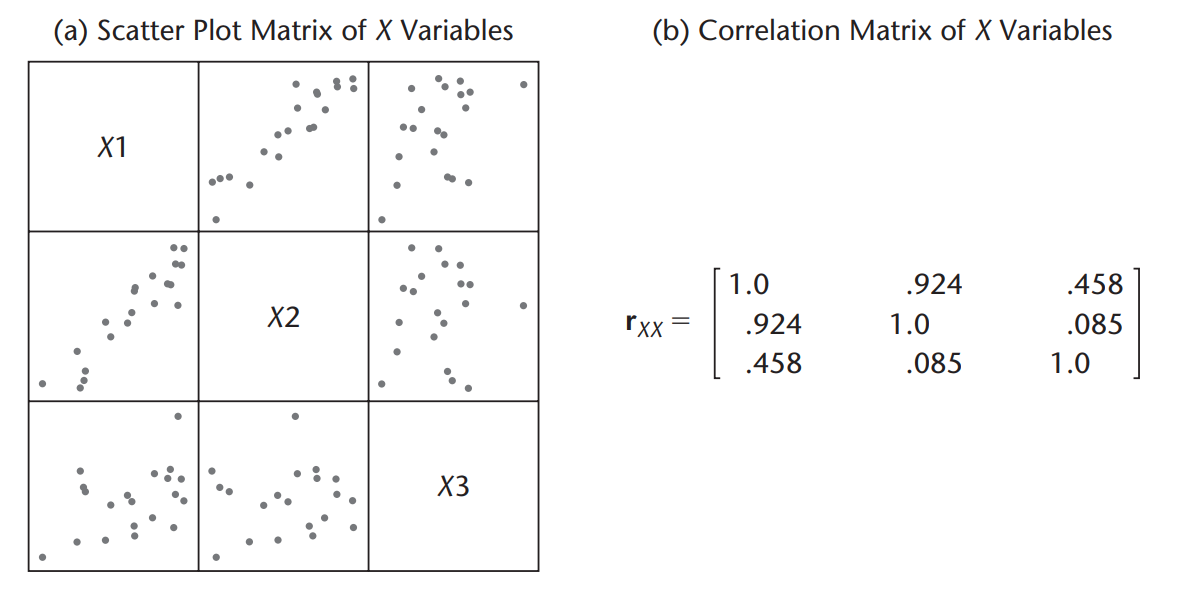
\includegraphics[width=1.0\textwidth]{figures/multicollinearity.png}

            \textit{$x_1$ and $x_2$ are highly correlated.}
        \end{center}
    \end{columns}

    \vspace{10pt}

    Reading: Chapter 7, Applied Linear Regression Models, Kutner, Nachtsheim, and Neter

  
\end{frame}

\begin{frame}{Autocorrelation}
    \begin{tblock}{}
        One of the standard assumptions in the regression model is that the error
terms $\epsilon_i$ and  $\epsilon_j$, associated with the ith and jth observations, are uncorrelated.
\begin{itemize}
    \item Correlation in the error terms suggests that there is additional information in the data that has not been exploited in the current model.
    \item When the
observations have a natural sequential order, the correlation is referred to as
\textbf{autocorrelation}. One example may be that the data is a timeseries data.
    \item Or, Adjacent residuals tend to be similar in both temporal and spatial dimensions. 
\end{itemize}
    \end{tblock}
    Reference: Chapter 9, Regression Analysis By Example Using R Ali S. Hadi, Samprit Chatterjee
\end{frame}

\begin{frame}{Example: Lack of independence}
        \begin{columns}
        \column{0.5\linewidth}
        \begin{center}
            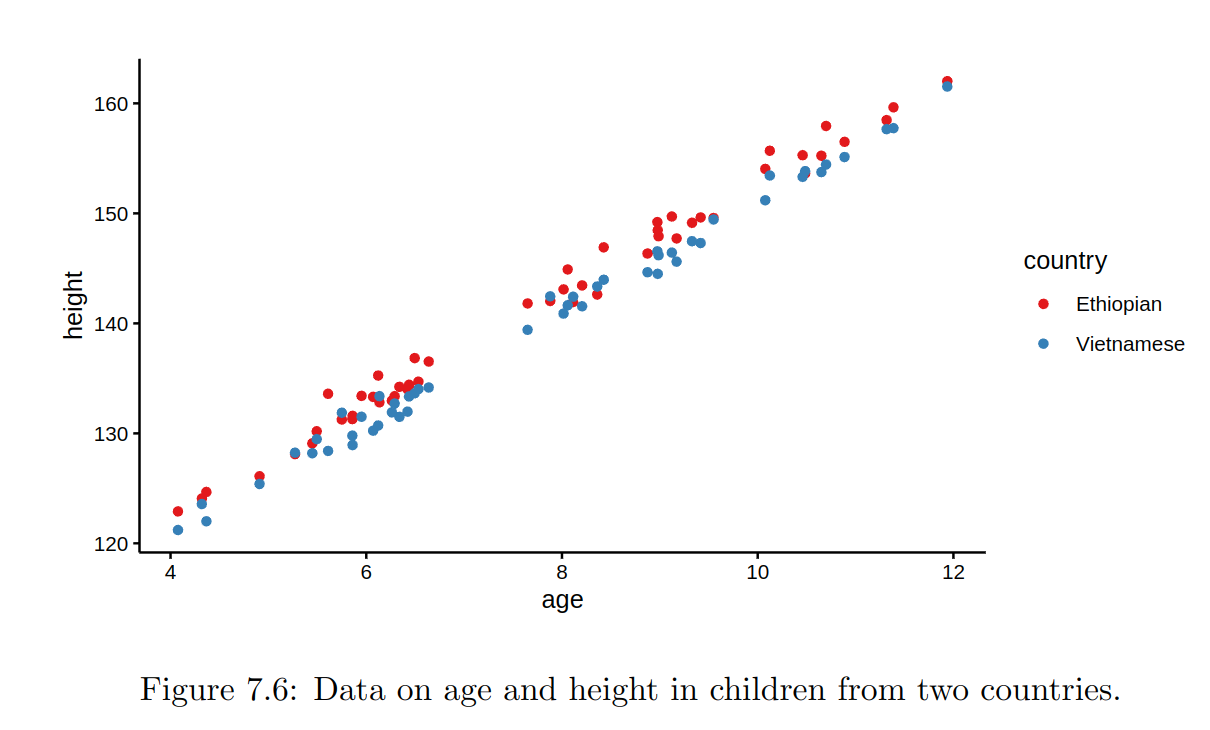
\includegraphics[width=1.0\textwidth]{figures/height_two_variables.png}

            \textit{Two groups stand out}
        \end{center}
        \column{0.5\linewidth}
        \begin{center}
            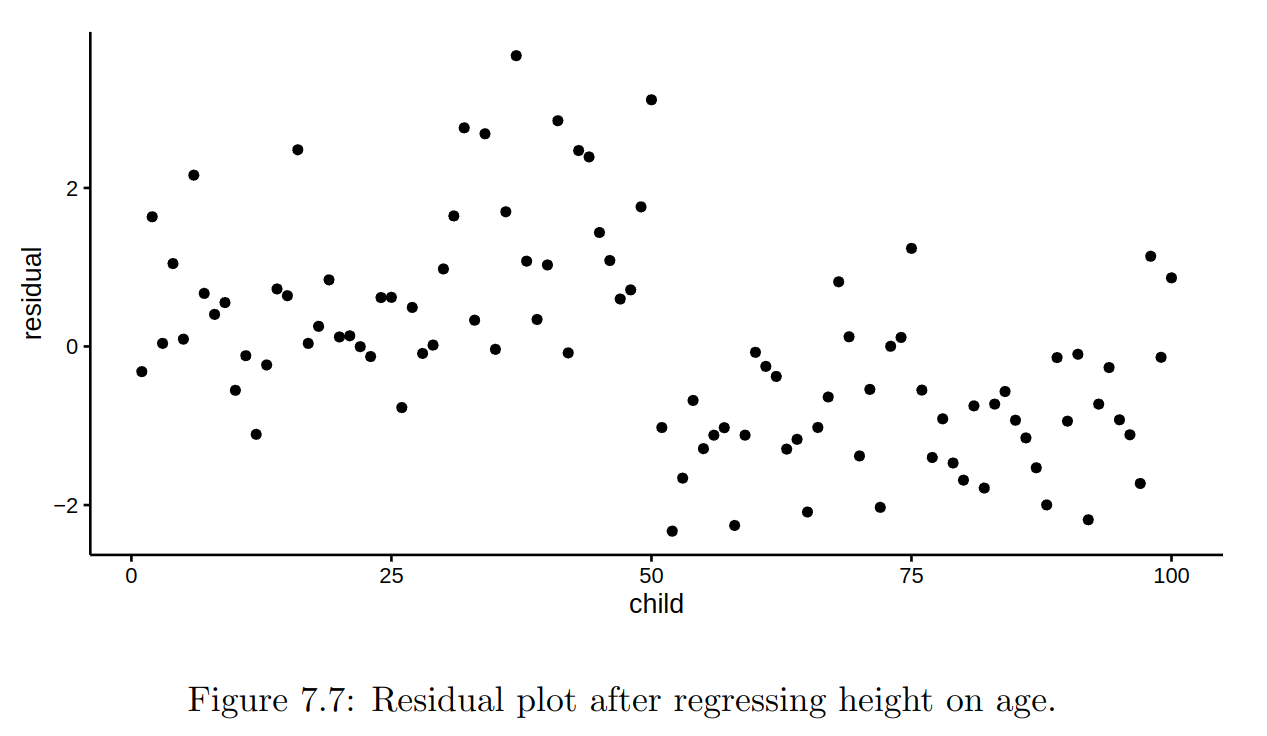
\includegraphics[width=1.0\textwidth]{figures/residual_plot_height_two_variables.png}

            \textit{Two groups stand out}
        \end{center}
    \end{columns}

    Reference: Analysing Data Using Linear Models. (2021). SM van den Berg
\end{frame}

\begin{frame}{Example: Deviation from Linearity}
        \begin{columns}
        \column{0.5\linewidth}
        \begin{center}
            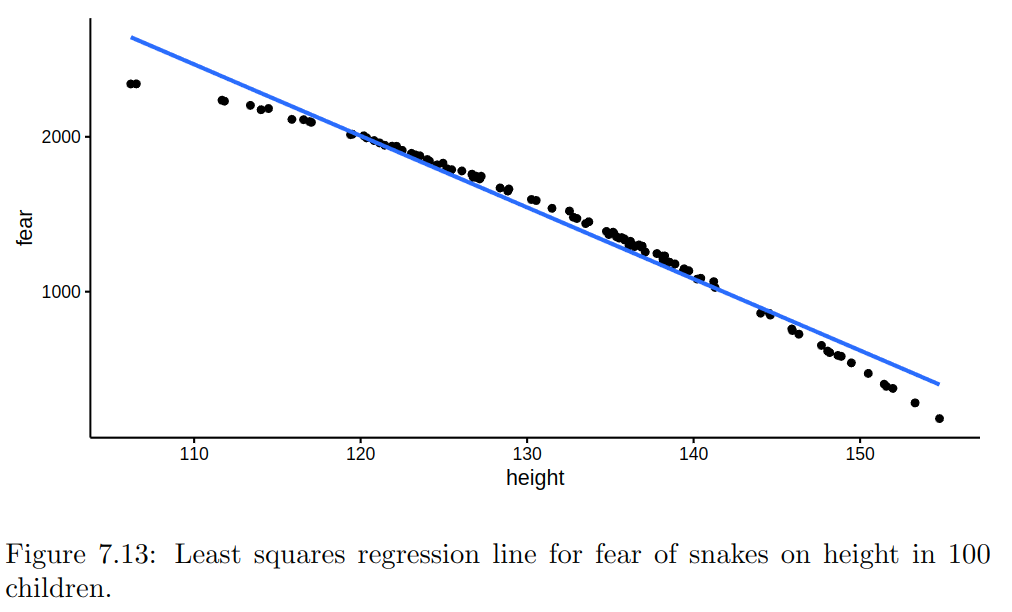
\includegraphics[width=1.0\textwidth]{figures/linearity_deviation.png}

            \textit{Deviation from Linearity}
        \end{center}
        \column{0.5\linewidth}
        \begin{center}
            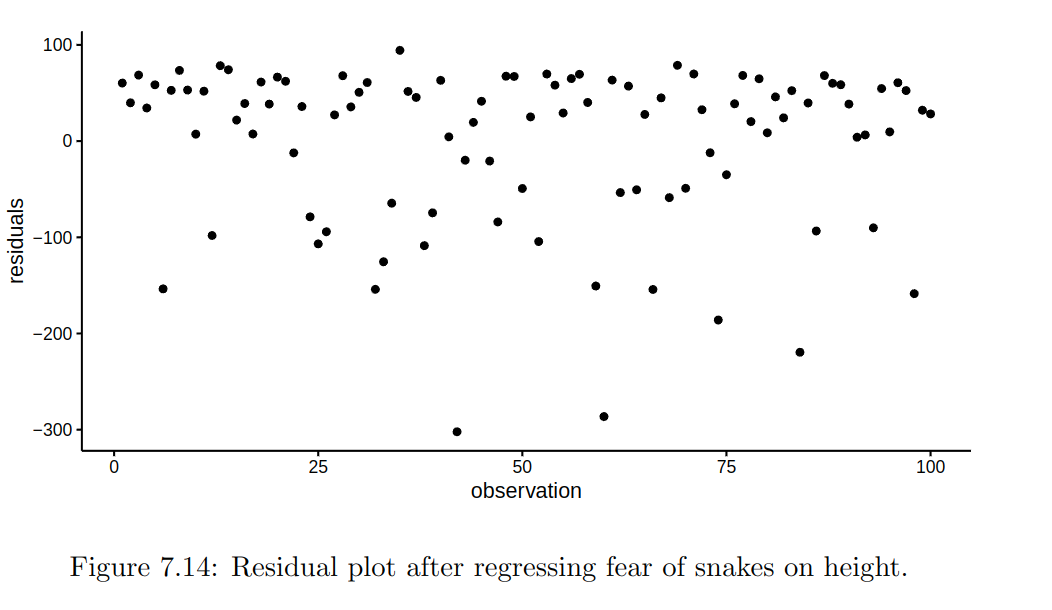
\includegraphics[width=1.0\textwidth]{figures/residual_plot_linearity_deviation.png}

            \textit{Residual Plot not symmetric, showing deviation from Linearity}
        \end{center}
    \end{columns}

      Reference: Analysing Data Using Linear Models. (2021). SM van den Berg
\end{frame}



\begin{frame}{Example: Deviation from Linearity}
        \begin{columns}
        \column{0.5\linewidth}
        \begin{center}
            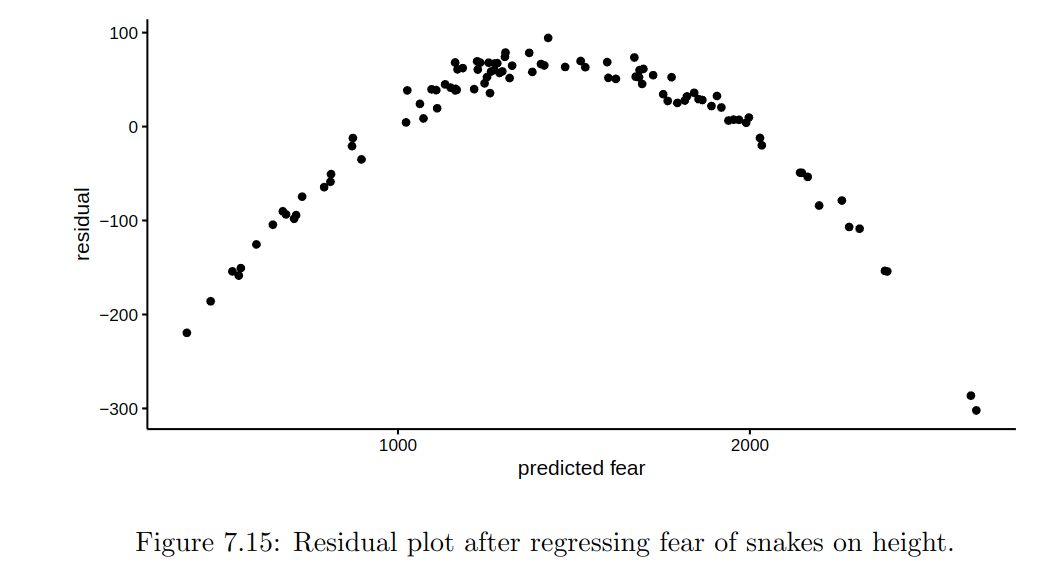
\includegraphics[width=1.0\textwidth]{figures/parabolic_residual.png}

            \textit{Deviation from Linearity}
        \end{center}
        \column{0.5\linewidth}
        \begin{center}
            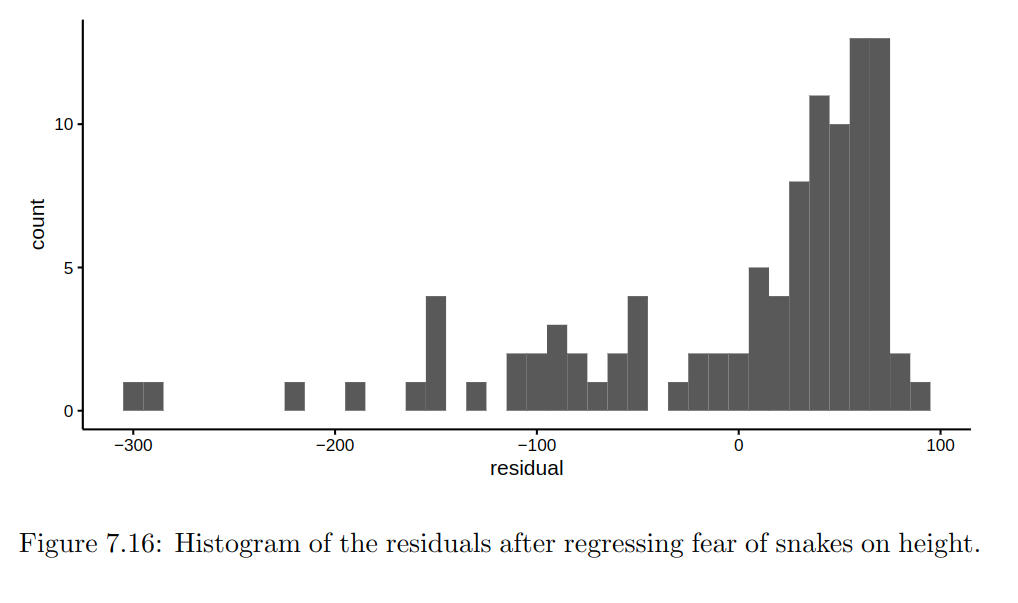
\includegraphics[width=1.0\textwidth]{figures/non_linear_histogram_residual.png}

            \textit{Residual Histogram not Gaussian}
        \end{center}
    \end{columns}

      Reference: Analysing Data Using Linear Models. (2021). SM van den Berg
\end{frame}

\begin{frame}{Homoscedasticity and Heteroscedasticity}


    \begin{tblock}{}
        The equal variance assumption is called \textbf{Homoscedasticity}. It means  constant variance of residuals across values of each predictor; in other words, residuals are evenly distributed
        throughout the regression line.
    \end{tblock}

    \vspace{10pt}

    \begin{center}
        On the other hand
    \end{center}

    \vspace{10pt}

    \begin{twilight}{}
        The condition of the error variance not being constant over all cases is called \textbf{Heteroscedasticity}. 
    \end{twilight}

\end{frame}

\begin{frame}{Heteroscedasticity in Data}
    

    \begin{cotton}{}
        Heteroscedasticity is inherent when the response in regression analysis follows a distribution in which the variance is functionally related to the mean. 
    \end{cotton}

    
    \pause 

    \vspace{10pt}

    \begin{golden}{}
        

        What probability distribution has variance as a function of mean?

        \pause

        Answer: Poisson distribution.
    \end{golden}

\end{frame}


\begin{frame}{Deviation from Homoscedasticity}

    If a dataset exhibits Homoscedasticity,  the scatterplot of the residuals shows a notable uniformity along the horizontal axis.

    \begin{center}
        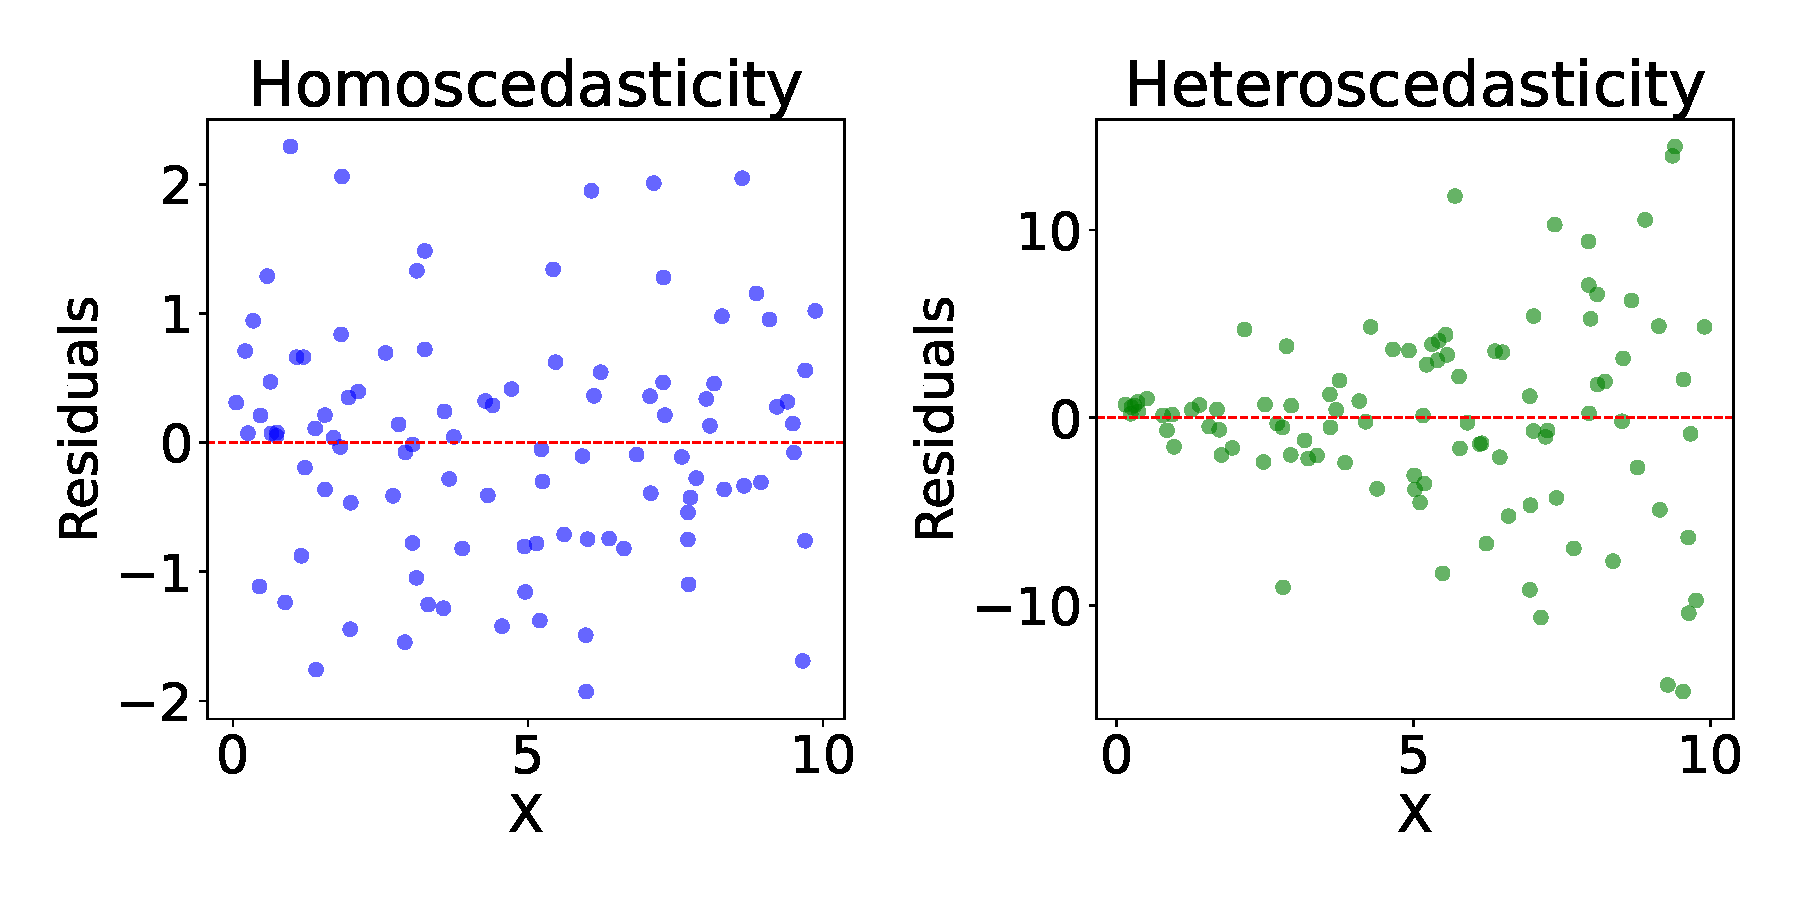
\includegraphics[width=0.6\textwidth]{figures/Homoscedasticity_vs_Heteroscedasticity.pdf}
    \end{center}
    
\end{frame}

\begin{frame}{Remedial Measures}

    \begin{itemize}
        \item Lack of Linearity: Use nonlinear regression
        \item Nonconstancy of Error Variance (Heteroscedasticity): Use weighted least square method (or Loess), sometimes transformation are effective too.
        \item Nonindependence of Error Terms: Autocorrelation may be present. Use transformed variables such as $y(t)_{tr} = y(t) - \rho y(t-1)$
        \item Nonnormality of Error Terms: Transform data. E.g. $y_{tr} = \sqrt{y}$, $x = \log(x)$, etc.
    \end{itemize}

     Reading: Chapter 3, Chapter 12, Applied Linear Regression Models, Kutner, Nachtsheim, and Neter
    
    
\end{frame}
% %%%%%%%%%%%%%%%%%%%%%%%%%%%%%%%%%%%%%%%%%%%%%%%%%%%%%
% \begin{sectionframe}{\faGroup}{Overfitting and Regularization}
% \end{sectionframe}



% %%%%%%%%%%%%%%%%%%%%%%%%%%%%%%%%%%%%%%%%%%%%%%%%%%%%%
% \begin{sectionframe}{\faGroup}{Transformations and Nonlinear Relationships}
% \end{sectionframe}

% %%%%%%%%%%%%%%%%%%%%%%%%%%%%%%%%%%%%%%%%%%%%%%%%%%%%%
% \begin{sectionframe}{\faGroup}{Generalized Linear Models (GLMs)}
% \end{sectionframe}


% %%%%%%%%%%%%%%%%%%%%%%%%%%%%%%%%%%%%%%%%%%%%%%%%%%%%%
% \begin{sectionframe}{\faGroup}{Robust Regression}
% \end{sectionframe}



    
      %------------------------------------------------
    
    \begin{frame}[containsverbatim]{Python Notebook}
    \begin{center}
    \small
    { \color{Red}{\url{https://github.com/rahulbhadani/CPE486586_FA26/blob/master/Code/CPE486586_Ch07_Advanced_Regression.ipynb}}}
    \end{center}
    \end{frame}
    
    %------------------------------------------------
    
    \begin{frame}
        \Huge{\centerline{\color{MediumBlue}\textbf{The End}}}
    \end{frame}

\end{document}